\documentclass[../../main.tex]{subfiles}

\begin{document}

    Category theory is the language needed to give simplicial/cyclic sets a simple definition. It is also an essential part of the language of algebraic topology. It begins with the elementary definitions of categories, functors, natural transformations and adjunctions.
        
    \begin{definition}
        A \defemph{category} $\cat{C}$ is a collection of \defemph{objects} $ob(\cat{C})$ and one of \defemph{arrows} or \defemph{morphisms} $arr(C)$ between objects. For every arrow $f$, there is an object $\domain{f}$, its \defemph{domain}, and $\codomain{f}$, its \defemph{codomain}. We say that an arrow points from $\domain{f}$ to $\codomain{f}$. For every pair of arrows $f, g$ such that $\domain{f} = \codomain{g}$ there is a composition of arrows $f \circ g$(often written omitting $\circ$) that fulfills the following axioms.
        
        \begin{enumerate}
            \item a) $\domain{fg} = \domain{g}$ \\
                b) $\codomain{fg} = \codomain{fg}$
            \item Associativity: (fg)h = f(gh) for all f,g,h where defined
            \item Identity: For every $c \in ob(C)$ there is an arrow $\idarrow[c]: c \to c$ such that $f \circ id_C = f$ and $g \circ id_c = g$ for all arrows $f, g$ where this composition is defined.
        \end{enumerate}
    \end{definition}
    
    Every category $\cat{C}$ has an associated category $\cat{C^{op}}$ formed by reversing all arrows in $\cat{C}$. Every statement in $\cat{C}$ can be made in $\cat{C^{op}}$ and is then called the \defemph{dual} statement. Its truth value is preserved.

    \begin{example}
        The category of topological spaces, usually denoted $\mathbf{Top}$, with objects being topological spaces and morphisms being continuous functions. A variant could be to limit spaces to compactly generated Hausdorff spaces usually referred to as $\mathbf{CGHaus}$.
    \end{example}

    \begin{definition}
        A (\defemph{covariant}) \defemph{functor} $\functor{F}: \cat{C} \to \cat{D}$ consists of a map of objects in $\cat{C}$ to objects in $\cat{D}$ and one map of morphisms in C to morphisms in D such that the following is fulfilled for all objects $a, b, c$ and arrows $g: a \to b, f: b \to c$.
        
        \begin{enumerate}
            \item $\domain{\functor{F}(f)} = \functor{F}(b), \codomain{\functor{F}(f)} = \functor{F}(c)$
            \item $\functor{F}(\idarrow[c]) = \idarrow[\functor{F}(c)]$
            \item $\functor{F}(fg) = \functor{F}(f) \circ \functor{F}(g)$ \label{cov}
        \end{enumerate}
        
        If \ref{cov} is reversed to $\functor{F}(fg) = \functor{F}(g) \circ \functor{F}(f)$, then $\functor{F}$ is \defemph{contravariant}.
    \end{definition}
    
    The contravariance/covariance in conjunction with the duality of categories can be somewhat disorienting. One can interchange a contravariant functor from a category, $\cat{C}$, to a covariant from the opposite, $\cat{C^{op}}$,.

    \begin{example}
        A few examples of functors include:
        \begin{itemize}
            \item the forgetful functor $G$, which forgets structure, e.g. $G:\mathbf{Grp}\to \mathbf{Set}$ taking a group to its underlying set
            \item simplicial set $X$, $X:\Delta\to \mathbf{Set}$, a contravariant functor
            \item geometric realization $\geom[\cdot]$, $\geom[\cdot]:\mathbf{sSet}\to \mathbf{CGHaus}$
        \end{itemize}
    \end{example}

    The two latter examples stated above will be further discussed in the next chapter, their concise statements are deceptive and require a more elaborate treatise. Somewhat easier to grasp is the following.
    
    Inside a given category $\cat{C}$, we often study some small, often finite, part of it. This is called a \defemph{diagram} in $\cat{C}$. Formally, an $\cat{I}$-shaped diagram $\functor{D}$ in $\cat{C}$ is a functor from an index category $\cat{I}$. If $\cat{I}$ is small, $\functor{D}$ is called a small diagram. Diagrams are a central concept in relation with them commuting. A commutative diagram is defined such that all directed paths with identical start and end points lead to the same results by composition. Commutative diagrams play the role in category theory that equations play in algebra (see Barr–Wells, Section 1.7).%check quote 
    
    If to a diagram $\functor{D}$ in $\cat{C}$, we add an object $e$ and arrows from $e$ to each object in $\functor{D}$ such that the resulting new diagram commutes, $e$ and the arrows form a \defemph{cone} over $\functor{D}$. A cone that is universal, in the sense that every other cone factors through it uniquely, is called a \defemph{limit} over $\functor{D}$. When a limit exist, it might not be unique. However, any other limit will be isomorphic to it. The dual notions are \defemph{cocones} and colimits. Important examples of limits are products are products, pullbacks, equalizers and terminal objects.
    
    \begin{figure}[H]
        \centering
        \begin{subfigure}[b]{0.5\textwidth}
            \centering
            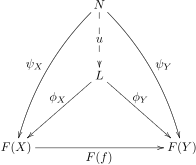
\includegraphics[scale=.65]{Functor_cone}
            \caption{}
        \end{subfigure}%
        ~ 
        \begin{subfigure}[b]{0.5\textwidth}
            \centering
            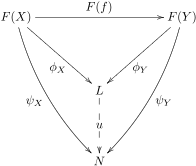
\includegraphics[scale=.65]{Functor_co-cone}
            \caption{}
        \end{subfigure}
        \caption{The cone/co-cone (left, right respectively) $(N,\Psi)$ factors/cofactors through the cone $(L,\phi)$ uniquely with $u$, the latter cone is then the limit/colimit}
    \end{figure}
    
    The categorical \defemph{product} can be easily defined in terms of limits. 
    
    \begin{definition}
        Given objects $\{c_i\}_{i \in I}$ in $\cat{C}$, their \defemph{product} is a limit over the diagram containing all $c_i$ and no arrows other than their identities.
    \end{definition}
    
    Examples of products is the cartesian product in $\cat{Set}$, the topological product in $\cat{Top}$ and the direct product in $\cat{Grp}$. In these categories, any set of objects has a product with these explicit constructions. The main reason of having the topological product defined the way it is(finitely many $O_i \neq X_i$) is to make it the categorical product in $\cat{Top}$. Would we not have this requirement(aka the box topology on $X$) it would merely be a cone over the discrete diagram of all $c_i$.
    
    As usual, there is a dual concept to products called a coproduct. Reverse all arrows in the definition of a product and you have a coproduct
    
    \begin{figure}[h]
        \centering
        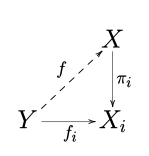
\includegraphics[scale=.7]{Cat_product}
        \caption{Diagram of a product. \textit{If Y is some object and for every i in I, $\pi_i:Y\to X_i$ is a morphism, then there exists a unique map $f:Y\to X$ such that for each i in I the diagram commutes.}}
        \label{fig:product}
    \end{figure}

    Examples of coproducts is the disjoint union in $\cat{Set}$ as well as its sibling, the disjoint union of topological spaces in $\cat{Top}$. This means that the cartesian product of topological spaces and the disjoint union of topological spaces are dual constructions. The same goes in $\cat{Set}$.
    
    One of the most important concepts in category theory is adjunctions. According to Saunders MacLane: \textit{“Adjoint functors arise everywhere.”}
    
    \begin{definition}
        Given $\functor{F}: \cat{D} \to \cat{C}$ and $\functor{G}: \cat{C} \to \cat{D}$, $\functor{F}$ is called \defemph{left adjoint} to $\functor{G}$ if for every $X \in C, Y \in D$ there is a bijection of hom-sets, $$\cat{C}(\functor{F}Y, X) \cong \cat{D}(Y, \functor{G}X)$$, which is natural in both $Y$ and $X$. $\functor{G}$ is then \defemph{right adjoint} to $\functor{F}$.
    \end{definition}
    
    An example of adjunctions are letting $\functor{G}$ be the forgetful functor mapping $\cat{Grp} \to \cat{Set}$. Its right adjoint is then $\functor{F}: \cat{Set} \to \cat{Cat}$ which sends a set $A$ to the free group on $A$. The bijections arises from the fact that a group homomorphism is completely described by its action on the generators.
    
    Another example is the abelianization functor $\functor{F}: \cat{Grp} \to \cat{Ab}$. It is left adjoint to the forgetful functor $\functor{G}: \cat{Ab} \to \cat{Grp}$. This is due to the fact that the commutator subgroup $[G, G]$ of any group $G$ needs to lie in the kernel of any homomorphism into an abelian group. This means that any such homomorphism will factor uniquely through the projection $G$ onto $G^{ab}$.
    
    For every set $X$, there are two canonical ways of defining a on it, the trivial topology and the discrete topology. These are in fact functors $\functor{F}: \cat{Set} \to \cat{Top}$. Assigning the discrete topology to $X$ by $\functor{F}$ will mean that any map \emph{from} it is continuous. Therefore we have a bijection between functions from $X$ into a given topological space $Y$ and continuous maps between X and $Y$. This means that this functor is left adjoint to the forgetful functor $\functor{G}: \cat{Top} \to \cat{Set}$. If instead we let $\functor{F}$ assign the trivial topology to $X$, every function \emph{to} $X$ is continuous and by the opposite argument $\functor{F}$ is right adjoint to $\functor{G}$.
    
    The \emph{Yoneda lemma} is perhaps the most important result in elementary category theory. It tells us something essential about representable functors which will be defined. In every category $\cat{C}$ and $A \in \cat{C}$ there is a covariant functor $h^A: \cat{C} \to \cat{Set}$, often denoted $\mathrm{Hom}_\cat{C}(A, -)$. It sends objects $X \mapsto \mathrm{Hom}_\cat{C}(A, X)$ and arrows $f \mapsto f \circ -$. In fact, 
    
    \begin{equation*}
        h^-: 
        \begin{cases}
            A \mapsto h^A \\
            f \mapsto f \circ -
        \end{cases}
    \end{equation*}
    
    is a contravariant functor called the \emph{Yoneda embedding}, $h^-: \cat{C}^{op} \to \cat{Set}^\cat{C}$.
    
    \begin{definition}
        A functor $\functor{F}: \cat{C} \to \cat{Set}$ is called \defemph{representable} if there is an object $A \in \cat{C}$ such that there is a natural isomorphism $h^A \cong \functor{F}$.
    \end{definition}
    
    \begin{theorem}[Yoneda lemma]
        Any functor $\functor{F}: \cat{C} \to \cat{Set}$ has a bijection for all $A \in C$ 
        $$\functor{F}(A) \cong \mathrm{Nat}(h^A, \functor{F})$$ 
        natural in $A$.
    \end{theorem}
    
    \begin{proof}
        Consider the following diagram of a natural transformation $\Phi$ between $h^A$ and $\functor{F}$ applied to $A$ and an arbitrary object $X \in C$. 
        
        \begin{figure}[H]
            \centering
            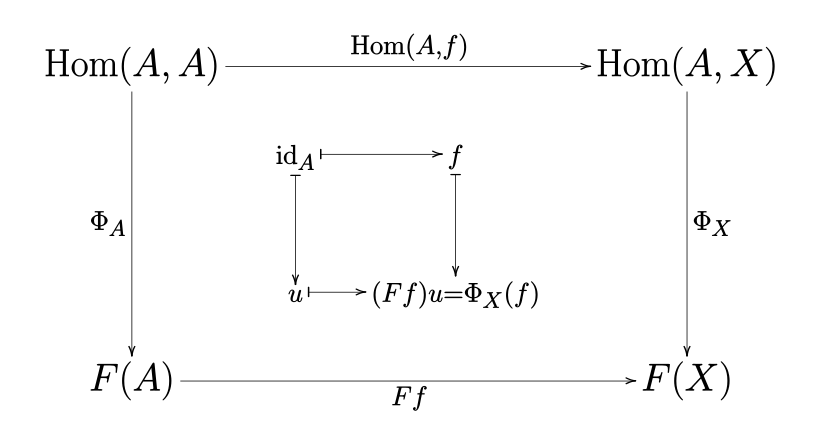
\includegraphics[scale=.35]{Yoneda_lemma_c}
            \caption{Diagram of natural transformation}
            \label{fig:boat1}
        \end{figure}

        Let $u$ be the action of $\Phi_A$ on $\idarrow[A]$. By looking at both ways of sending $\idarrow[A]$ to $\functor{F}(X)$ it is realized that the action of $\Phi_X$ on any $f \in \mathrm{Hom}(A, X)$ is given by 

        \begin{equation}
            \Phi_X(f) = \functor{F}f(u)
        \end{equation}
        
        This means that $\Phi$ is completely determined by its action on the identity which can take on any value in $\functor{F}(A)$.
    \end{proof}

\end{document}